 \begin{flushleft}
{\Huge Snapsvisor\\}
\vspace{1 cm}
{\Large
I vårt avlånga land står många olika sorters snaps att finna, vissa godare
än andra. Självklart väljer var person snaps efter eget tycke, men en snaps som innehar en viss särställning gentemot andra är
Bäska droppar. Trots sin något avancerade smak har den blivit så populär
att den länge varit ett givet inslag på de flesta Chalmersfester. Viss varsamhet bör
dock iakttagas vid intagande av snapsen, då det är lätt att bli styv i
korken efter ett alltför ymnigt pokulerande. 
}
\end{flushleft}
\vspace{2cm}
\begin{center}
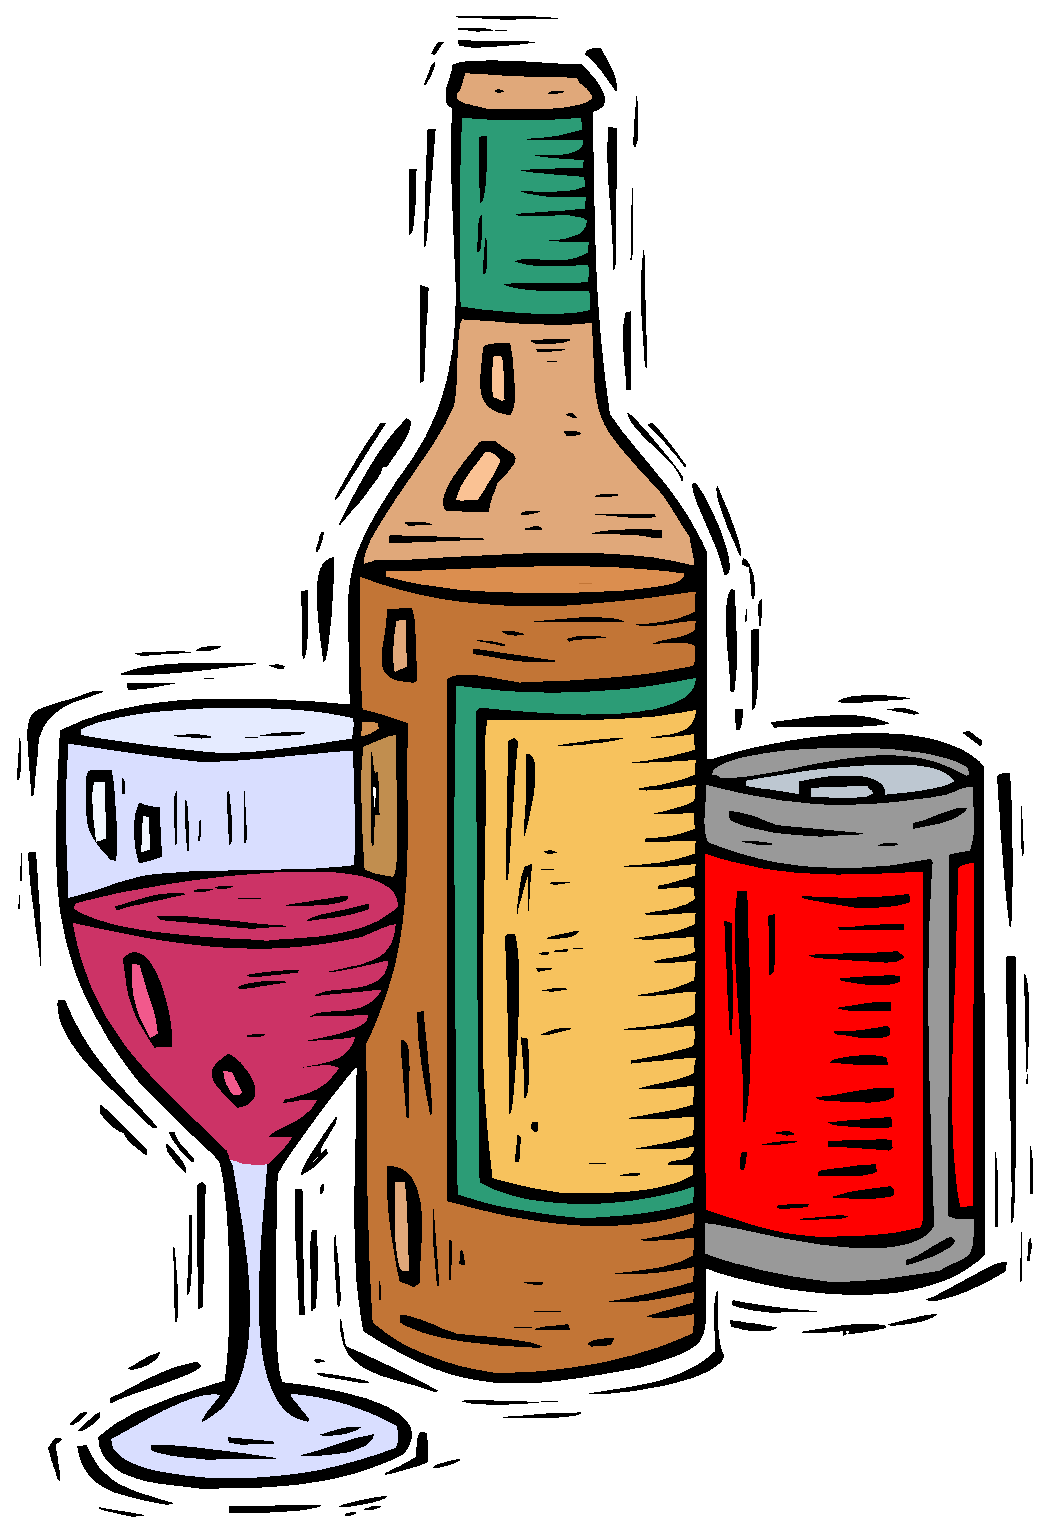
\includegraphics[width=6cm]{bilder/8.eps}
\end{center}

\newpage

\begin{song}{Helan går}{helan}
\begin{vers}
Helan går,\\
sjung hoppfadderallanlallanlej!\\
Helan går,\\
sjung hoppfadderallanlej!\\
Den som inte helan tar,\\
han heller inte halvan får.\\
Helan går...(drycken inmundigas)\\
sjung hoppfadderallanlej!\\
\end{vers}
\end{song}


\begin{song}{Hell and gore}{hellandgore}
\mel{Helan går}   
\begin{vers}
Hell and gore\\
Chunk happ father Allan-lallan-lay.\\
Hell and gore\\
Chunk happ father Allan-lay.\\
Oh handsome in the hell and tar\\
hand hell are in the half and four.\\
Hell and gore...(Take the booze)\\
Chunk happ father Allan-lay!\\
\end{vers}
\end{song}

\newpage

\begin{song}{Halvan}{halvan}
\begin{vers}
//: Hur länge skall på bordet\\
den lilla halvan stå?\\
Skall snart ej höras orden:\\
Nu halvan går, låt gå. ://\\
//: Det ärvde vikingsinne\\
till supen trår igen,\\
och helans trogna minne\\
i halvan går igen. ://\\
\end{vers}
\end{song}

\begin{song}{Mera brännvin}{merabrannvin}
\mel{Internationalen\\ Text: Hans Dahlborg}
\begin{vers}
Mera brännvin i glasen\\
mera glas på vårt bord.\\
Mera bord på kalasen\\
mer kalas på vår jord.\\
\end{vers}
\begin{vers}
Mera jordar med måne\\
mera måne i Mars.\\
Mera marscher mot Skåne\\
mera Skåne gubevars.\\
\end{vers}
\end{song}

\newpage

\begin{song}{Måsen}{masen}
\mel{När månen vandrar på fästet blå}
\begin{vers}
Det satt en mås på en klyvarbom,\\
och tom i krävan var kräket.\\
Och tungan lådde vid skepparns gom,\\
där han satt uti bleket.\\
Jag vill ha sill, hördes måsen rope,\\
och skepparn svarte: Jag vill ha OP,\\
om blott jag får, om blott jag får.\\
\end{vers}

\begin{vers}
Nu lyfter måsen från klyvarbom,\\
och vinden spelar i tågen.\\
OP:n svalkat har skepparns gom,\\
jag önskar blott att jag såg'en.\\
Så nöjd och lycklig den arme saten,\\
han sätter storsegel, den krabaten.\\
Till sjöss han far, och halvan tar.\\
\end{vers}

\begin{vers}
Den mås som satt på en klyvarbom,\\
Den är nu död och begraven,\\
Och skepparn som drack en flaska rom,\\
han har nu drunknat i haven.\\
Så kan det gå om man fått för mycket,\\
Om man för brännvin har fattat tycke.\\
Vi som har kvar, vi resten tar.\\
\end{vers}
\end{song}

\newpage

\begin{song}{Månen}{manen}
\mel{När månen vandrar på fästet blå}
\begin{vers}
När månen vandrar sin tysta ban\\
och tittar in genom rutan.\\
Då tänker jag att på ljusa dan\\
så kan jag klara mig utan.\\
Då kan jag klara mig utan måne,\\
men utan renat och utan Skåne...\\
Det vete fan, de vete fan.\\
\end{vers}
\end{song}

\begin{song}{Moosen}{moosen}
\mel{När månen vandrar på fästet blå}
\begin{vers}
Det satt en älg i en klyvartopp,\\
förklädd i älgjaktens månad.\\
Han var befjädrad till horn och kropp;\\
och skepparn blev rätt förvånad.\\
"Jag är en mås, goa skepparn!", ljög den\\
förklädda älgen och sedan flög den.\\
Mjukt landa den,
på skepparen.\\
\end{vers}
\end{song}

\begin{song}{Mesen}{mesen}
\mel{När månen vandrar på fästet blå}
\begin{vers}
Det satt en mes i en klyvarmast,\\
där sågs han ragla och svaja.\\
För trots att frön var hans ända last\\
var han full som en kaja.\\
"Vad har du gjort?", hördes skepparn stöna,\\
och mesen svarte: "Jag rökte fröna,\\
i egen holk, i egen holk."\\
\end{vers}
\end{song}

\begin{song}{Musen}{musen}
\mel{När månen vandrar på fästet blå}
\begin{vers}
Det satt en mus i en hushållsost,\\
och åt och åt utan måtta\\
tills osten blev till en mushåls-ost\\
och han en klotformad råtta.\\
"Så bra" sa musen, "att va en fettboll\\
nu kan jag rulla med hast år rätt håll.\\
Ostindien! Ostindien!"\\
\end{vers}
\end{song}

\newpage

\begin{song}{Porthos visa}{porto}
\mel{Annie get your gun\\Ur KTHs Bergsspex, De tre musketörerna, 1960}
\begin{vers}
Jag vill ut å gasqua,\\
var faan är min flaska,\\
vem i helvete stal min butelj?\\
Skall törsten mig tvinga,\\
en TT börja svinga?\\
Nej för fan bara blunda och svälj.\\
\end{vers}
\begin{vers}
Vilken smörja! Får jag spörja?\\
Vem för fan tror att jag är en älg?\\
\end{vers}
\begin{vers}
Till England vi rider\\
och sedan vad det lider,\\
träffar vi välan på någon pub.\\
Och där skall vi festa,\\
blott dricka av det bästa\\
utav whisky och portvin,\\
jag tänker gå hårt in\\
för att prova på rubb och stubb.\\
\end{vers}
\begin{vers}
Rubb och stuubb, rubb och stuubb\\
Rubb och stubb, rubb och stubb, rubb och stubb!\\
\end{vers}
\end{song}

\newpage

\begin{song}{Jag har aldrig var't på snusen}{snusen}
\mel{O hur saligt att få vandra}
\begin{vers}
Jag har aldrig var't på snusen,\\
aldrig rökat en cigarr. Halleluja!\\
Mina dygder äro tusen,\\
inga syndiga laster jag har.\\
Jag har aldrig sett nåt naket,\\
inte ens ett litet nyfött barn.\\
Mina blickar går mot taket\\
därmed undgår jag frestarens garn.\\
\end{vers}
\begin{vers}
Halleluja, halleluja...\\
\end{vers}
\begin{vers}
Bacchus spelar på gitarren,\\
Satan spelar på sitt handklaver.\\
Alla djävlar dansar tango\\
säg vad kan man väl önska sig mer?\\
Jo! Att alla bäckar vore brännvin\\
Mölndalsån var fylld med Bayerskt öl,\\
konjak i varenda rännsten\\
och punsch i varendaste pöl!\\
\end{vers}
\begin{vers}
Halleluja, halleluja...\\
\end{vers}
\end{song}
%Bortkommenterad 2014
%\newpage

%\begin{song}{Handelsvisan}{handelsvisan}
%\mel{O hur saligt att få vandra}
%\begin{vers}
%Jag vill inte gå på Handels\\
%inte tenta företagsekonomi.\\
%Deras IQ, den är Mandels.\\
%Och förståndet, det har gjort sorti.\\
%De har jätteusla snören,\\
%%till sitt jätteusla draperi.\\
%De kan bara räkna ören.\\
%Hela skolan är ett enda aperi.\\
%\end{vers}
%\begin{vers}
%%Handels är skit - Jag vill ej dit...\\
%\end{vers}
%\begin{vers}
%Mammons pojkar är de alla.\\
%Pappas flickor är de likaså.\\
%Går och tror att de är balla.\\
%Fast de inget alls ju förstå.\\
%Nej, hela Handels borde rivas.\\
%Detta anser hela vårat lag.\\
%Ja, då skulle Emil trivas,\\
%uppå denna Handels ljuva domedag.\\
%\end{vers}
%\begin{vers}
%Åh vilket drag - På denna dag...\\
%\end{vers}
%\end{song}

\newpage

\begin{song}{Lyftet}{lyftet}
\mel{Ding dong merrily on high\\ Ur Götheborgs Medicinarspex Nero II, 1968}
\begin{vers}
Lyft ditt välförsedda glas,\\
det är en härlig börda.\\
Nu har grabbarna kalas,\\
vi segern snart skall skörda!\\
\end{vers}
\begin{vers}
//: Ding, dingedingeding,\\
dingedingeding,\\
dingedingeding, dong, dong.\\
Imorgon är det lördag! ://\\
\end{vers}
\begin{vers}
Sätt nu glaset till din mun,\\
se döden på dig väntar.\\
Nu har grabbarna kalas,\\
hör liemannen flämta!\\
\end{vers}
\begin{vers}
//: Ding, dingedingeding,\\
dingedingeding,\\
dingedingeding, dong, dong\\
Begravningsklockor klämtar! ://\\
\end{vers}
\end{song}

\newpage

\begin{song}{Ratatata}{rattata}
\mel{Fritt efter Povel Ramel}
\begin{vers}
Att dricka brännvin är en sed\\
som ingen har oss lärt.\\
Från början vi ej kunde,\\
men det var blott temporärt.\\
Sen lärde vi oss själva,\\
och nog var det värt besvär't.\\
Tutilurenbom tutidalenpang\\
nog var det värt besvär't.\\
\end{vers}
\begin{vers}
//: Rattataa, så tar vi oss en tuting\\
rattataa, med mycket brännvin i\\
rattata, rattatata, dricka brännvin gillar ja'\\
för jag blir så glad ida'! ://\\
\end{vers}
\end{song}

\begin{song}{Nu tar vi den}{nutarviden}
\mel{O Tannenbaum}
\begin{vers}
//:Nu tar vi den :// 4ggr i tre verser.\\
\end{vers}
\end{song}

\newpage

\begin{song}{23:an}{tjutrean}
\mel{Oh, Susannah}
\begin{vers}
Jag har vandrat ifrån Äppelbo
igenom mo och träsk.
Enda målet med min resa var
att finna än en Bäsk.
\end{vers}
\begin{vers}
O 23:an hör ropet från mitt bröst.
Hör mitt gnäll, mitt gny,
mitt sorgeskri,
min strupes torra röst.
\end{vers}
\end{song}



\begin{song}{O.P. river}{opriver}
\mel{Old man river}
\begin{vers}
O.P. river ja, O.P. river\\
var gång jag lenat min hals med Renat\\
jag sagt med iver att O.P. river\\
långt ner, långt ner.\\
\end{vers}
\begin{vers}
Mången glädes när han fått sädes\\
och fattighjonet ses le mot kronet,\\
men faktum bliver att O.P. river\\
långt ner, långt ner.\\
\end{vers}
\end{song}

\begin{song}{Byssan lull}{byssanlull} 
\mel{Byssan lull}
\begin{vers}
Byssan lull snart så blir du lite full.\\
Du får tre jamare på festen.\\
Den ene får du nu, den andre får du sen,\\
men den tredje får du smyga fram ur västen.\\
\end{vers}
\end{song}

\newpage

\begin{song}{Solen}{solen}
\mel{Camptown Ladies}
\begin{vers}
Solen den går upp och ner doda, doda.\\
Jag skall aldrig supa mer, hej doda dej.\\
Hej doda dej, hej doda dej.\\
Jag skall aldrig supa mer, hej doda dej.\\
\end{vers}
\begin{vers}
Men detta det var inte sant doda, doda.\\
I morgon gör jag likadant, hej doda dej.\\
Hej doda dej, hej doda dej.\\
I morgon gör jag likadant, hej doda dej.\\
\end{vers}
\begin{vers}
Chalmers är ett jävla skit, doda doda.\\
Jag skall aldrig mer gå dit, hej doda dej.\\
Hej doda dej, hej doda dej\\
Jag skall aldrig mer gå dit,\\
hej doda dej.\\
\end{vers}
\begin{vers}
Men detta det var inte sant...\\
\end{vers}
\end{song}


\newpage

\begin{song}{Än en gång däran}{anengang}
\mel{Fritt efter Evert Taube}
\begin{vers}
Än en gång däran bröder,\\
än en gång däran,  \\
följom den urgamla seden.   \\
Intill sista man bröder,\\
intill sista man,\\
trotsar vi hatet och vreden.\\
Blankare vapen sågs aldrig i en här,\\
än dessa glasen, kamrater, i gevär!\\
Än en gång däran bröder,\\
än en gång däran,  \\
Svenska hjärtans djup, här är din sup!\\
\end{vers}
\begin{vers}
Livet är så kort bröder,\\
livet är så kort.\\
lek det ej bort, nej var redo.\\
Kämpa mot allt torrt bröder,\\
kämpa mot allt torrt. \\
Tänk på de gamble som skredo\\
fram utan tvekan i floder av champagne,\\
styrkta från början av brännvin från vårt land.\\
Kämpa mot allt torrt bröder,\\
kämpa mot allt torrt.\\
Svenska hjärtans djup, här är din sup!\\
\end{vers}
\end{song}

\newpage

%\begin{song}{Invers aptit}{inversaptit}
%\mel{Nu tändas tusen juleljus}
%\begin{vers}
%Nu fyllas många magar små\\
%av iskall renad sprit.\\
%Men några kastar åter opp.\\
%Det är invers aptit.\\
%\end{vers}
%\end{song}

\begin{song}{Glädjetåren}{gladjetaren}
\mel{Familjen Flinta\\ ur Chalmersspexet Victoria, 1986}
\begin{vers}
Helan, sköna Helan!\\
Ljuva droppar i en glädjetår!\\
\end{vers}
\begin{vers}
Helan, fegt att dela'n!\\
Den ger styrka och du bättre mår!\\
\end{vers}
\begin{vers}
Men spriten, dödar långsamt har man spått.\\
Tur det, för vi har ju knappast brått!\\
\end{vers}
\begin{vers}
Livet, det är givet.\\
Det skall levas fyllt av glädje, \\
ni måste medge:\\
Bäst är en glädjetår!\\
\end{vers}
\end{song}

\begin{song}{Tänk om jag hade}{omjaghade}
\mel{Hej tomtegubbar}
\begin{vers}
//: Tänk om jag hade lilla nubben\\
uppå ett snöre i halsen ://\\
Jag skulle dra den upp och ner,\\
så att den kändes som många fler.\\
Tänk om jag hade lilla nubben\\
uppå ett snöre i halsen.\\
\end{vers}
\end{song}
\newpage

\begin{song}{Vikingen}{vikingen}
\mel{When Johnny Comes Marching Home\\från E-LTH, Sångarstriden 1981}
\begin{vers}
En viking älskar livets vann\\
Hurra, hurra!\\
Det hastigt i hans svalg försvann\\
Hurra, hurra!\\
Till kalv, till oxe, till fisk och till fläsk\\
När kärringen bara dricker läsk,   \\
ja då vill alla vikingar ha en Bäsk.\\
\end{vers}
\begin{vers}
När Bäsken småningom är slut\\
Tragik, tragik! \\
Då bäres varje viking ut\\
som lik, sej lik.\\
Och sen när vi vaknar vi sjunger en bit,\\
och korkar upp en Skånes Aquavit\\
Skål för alla vikingar som kom hit!\\
\end{vers}
\end{song}

\begin{song}{En liten fyllhund}{fyllhund}
\mel{Mors lilla Olle}
\begin{vers}
En liten fyllhund på krogen satt\\
rosor på kinden, men blicken var matt\\
läpparna små, liksom näsan var blå\\
bara jag kunde så skulle jag gå.\\
\end{vers}
\end{song}

\newpage

\begin{song}{Vodka vodka}{vodkavodka}
\mel{Stenka Rasin}
\begin{vers}
Vodka, vodka vill jag dricka\\
Jag vill äta kaviar.\\
//: Jag vill älska russki flicka\\
jag vill spy i samovar. ://\\
\end{vers}
\begin{vers}
Whiskey, whiskey will jag dricka.\\
Jag vill äta baked beans.\\
//:Jag will älska US flicka.\\
Jag will spy på mina jeans.://\\
\end{vers}
\begin{vers}
Falu brännvin vill jag dricka\\
Jag vill äta falukorv.\\
//: Jag vill älska falu flicka   \\
jag vill spy i faluån. :/\\
\end{vers}
\begin{vers}
	Bäska droppar vill jag dricka.\\
	Jag vill äta en baguette.\\
	//:Jag vill älska Chalmersflicka.\\
	Jag vill spy på alla sätt://\\
\end{vers}
\end{song}

\newpage

\begin{song}{Jag är lapp och jag har lite renat}{literenat}
\mel{Vid foten av fjället}
\begin{vers}
Jag är lapp och jag har lite renat\\
det är hemgjort, ja tacka för det\\
ty att köpa blir dyrt så förbenat\\
för då kommer ju frakterna te.\\
\end{vers}
\begin{vers}
Här vid foten av snöklädda fjället\\
finns en plats dit jag drar varje vår\\
det är faktiskt nåt särskilt med stället\\
det är där apparaten min står.\\
\end{vers}
\begin{vers}
Men en natt var där odjur i trakten\\
där var skära elefanter och möss.\\
Och till trolltrummans ljud upptogs jakten\\
till apparaten så sa jag adjöss.\\
\end{vers}
\begin{vers}
Men när jag kom tillbaka till fjället\\
av apparaten fanns inte ett spår\\
ty se länsman han hittade stället\\
och i finkan så ensam jag går.\\
\end{vers}
\end{song}

\newpage

\begin{song}{En ters}{enters}
\mel{Schottis på Valhall}
\begin{vers}
Upp med glaset Bror både liten och stor\\
som har plats här vid bordet ikväll.\\
Just till denna vers ska vi taga en ters\\
vi får hämta ännu en putell.\\
Nog blir näsan röd utav denna mjöd\\
men kulören den gör ej ett skvatt.\\
Nu står Tersen på tur,\\
och den dricker vi ur\\
Det är fest här i huset i natt.\\
\end{vers}
\end{song}

\begin{song}{Nubben walk}{nubbenwalk}
\mel{Lamberth Walk}
\begin{vers}
Jag kan ännu skilja på tak och golv\\
Två gånger sex och en halv är tolv\\
Två gånger tre är sju\\
Hur i helvete räknar jag nu\\
Hej!\\
Nubbar man för lite blir livet torrt\\
Nubbar man för mycket blir livet kort\\
Nej, gör som jag\\
Nubba lite varje dag\\
Hej!\\
\end{vers}
\end{song}

\newpage

\begin{song}{En bidragstagare}{bidragstagare}
\mel{En Sockerbagare\\text Roger Melander}
\begin{vers}
En bidragstagare här bor i staden\\
han dricker brännvin mest hela dagen\\
han dricker öl och han dricker vin\\
och kallas allmänt för fyllesvin\\
\end{vers}
\end{song}

\begin{song}{En gång i månan}{engangimanan}
\mel{Mors lilla Olle}
\begin{vers}
En gång i månan är månen full,\\
aldrig vi sett honom ramla omkull.\\
Stum av beundran hur mycket han tål\\
höjer vi glasen och utbringar skål!\\
\end{vers}
\begin{vers}
Höjen nu glasen och dricken ur.\\
Nu, kära bröder, står helan (halvan) i tur.\\
Nubben den giver oss ny energi,\\
Säkert den minskar vårt livs entropi.\\
\end{vers}
\end{song}

\newpage

\begin{song}{Dom som är nyktra}{nyktra}
\mel{Du är den ende\\Text: Håkan 'Sebbe' Jakobsson}
\begin{vers}
(moll) Dom som är nyktra har inte så roligt,\\
dom har bara ansvar och inte nå't\\
tjolitt-an-lej-faderulla,\\
men vi som är fulla\\
vi har bara kul nästan jämt.\\
\end{vers}
%\begin{vers}
%	Det sägs att en mänska kan va utan brännvin.\\
%	Det stämmer kanhända men se blott på den min\\
%	som pryder en absolutist den är jävligt trist,\\
%	därför så sjunga vi så:\\
%\end{vers}
%\begin{vers}
%	De som är nyktra...
%\end{vers}
\begin{vers}
(dur) Det gör det samma var vi må va' gäster\\
Ja till och med lanthushållningssällskapsfester\\
kan uthärdas med eau-de-vie,\\
som får månda'n att bli\\
blott en vag utopi.\\
\end{vers}
\end{song}
%tillagd 2014 från F på Lund
\begin{song}{Avundsjuk visa}{avundsjukvisa}
\mel{En sockerbagare}
\begin{vers}
En sockerdrickare finns på kalaset.\\
Han dricker Champis det lilla aset.\\
Han dricker Pommac och 7-up\\
och när jag deckar så får han napp.\\
\end{vers}
\end{song}

\newpage

\begin{song}{Full ida'}{fullida}
\mel{Clementine}
\begin{vers}
Full ida' och full i morgon,\\
så ser livet ut för oss.\\
Vi ska göra som alla andra,\\
vi ska supa och vi ska slåss.\\
\end{vers}
\begin{vers}
Och på vår gravsten, och på vår gravsten,\\
ska det skrivas på latin.\\
Här inunder denna sten\\
ligger det ett fyllesvin.\\
\end{vers}
\begin{vers}
Och dessa maskar, och dessa maskar,\\
dom ska äta av vår kropp.\\
Dom ska känna alkoholen,\\
dom ska aldrig komma opp.\\
\end{vers}
\end{song}

\begin{song}{Mitt lilla lån}{mittlillalan}
\mel{Hej tomtegubbar}
\begin{vers}
//: Mitt lilla lån det räcker inte\\
det går till öl och till brännvin ://\\
Till öl och brännvin går det åt,\\
och till en kursbok emellanåt.\\
Mitt lilla lån det räcker inte\\
det går till öl och till brännvin\\
\end{vers}
\end{song}

\newpage

\begin{song}{Spritbolaget}{spritbolaget}
\mel{Snickarboa}
\begin{vers}
Till spritbolaget ränner jag\\
och bankar på dess port.\\
Jag vill ha nå't som bränner bra\\
och gör mig sketfull fort.\\
Expediten sade: Godda'.\\
Hur gammal kan min herre va'?\\
Har du nå't leg, ditt fula drägg?\\
Kom hit igen när du fått skägg!\\
\end{vers}
\begin{vers}
Nej, detta var ju inte bra,\\
jag ska bli full ikväll.\\
Då plötsligt en idé fick jag,\\
dom har ju sprit på Shell.\\
Många flaskor stod där på rad,\\
så nu kan jag bli full och glad.\\
Den röda drycken åkte ner.\\
Nu kan jag inte se nåt mer!\\
\end{vers}
\end{song}

\newpage

\begin{song}{Båtvisa}{batvisa}
\mel{Jazzgossen}
\begin{vers}
Och så kommer det en ångbåt,   \\
som säger: Tuuuuuut!\\
\end{vers}
\begin{vers}
Å så kommer det en ubåt,\\
som säger: Gurgeliblurgeliglur!\\
\end{vers}
\end{song}

\begin{song}{Oasen}{oasen}
\mel{British Grenadiers, trad\\Ur Chalmersspexet Tutankamon, 1980}
\begin{vers}
Som ökensand känns strupen ibland,\\
och man orkar inte bära hand.\\
Fy Farao, ej rast eller ro,\\
man blir nykter som en helig ko.\\
\end{vers}
\begin{vers}
//: Men till och med en mumie\\
får ryckningar i sarkofagen.\\
Det spritter i kistan\\
när örat hör listan\\
på supar som bjudes på vår gasque! ://\\
Hej skål!\\
\end{vers}
\end{song}

\newpage



\begin{song}{Jag skall festa}{jagskallfesta}
\mel{Bamse\\från D-LTH, sångarstriden -87}

\begin{vers}
Jag skall festa, ta det lugnt med spriten\\
ha det roligt utan att va' full.\\
Inte krypa runt med festeliten,\\
ta det varligt för min egen skull.\\
\end{vers}
\begin{vers}
Först en öl i torra strupen,\\
efter det så kommer supen,\\
i med vinet, ner med punschen\\
sist en groggbuffé.\\
\end{vers}
\begin{vers}
Jag är skitfull, däckar först av alla\\
missar festen, men vad gör väl de'?\\
Blandar hejdlöst öl och gammal filmjölk,\\
kastar upp på bordsdamen breve'!\\
\end{vers}
\end{song}

\begin{song}{1 2 75 6 7}{etttva}
\mel{Ritsch, ratsch}
\begin{vers}
1 2 75 6 7 75 6 7 75 6 7\\
3 2 75 6 1 43 7 1 92\\
103 102 101 105 6 19 47\\
19 18 17 16 15 14 13 11\\
16 17 18 19 13 55\\
\end{vers}
\end{song}

\newpage

\begin{song}{Lille Olle}{lilleolle}
\mel{Katuschka}
\begin{vers}
Lille Olle skulle gå på disko,  \\
men han hade inte någon sprit. \\
Lille Olle skaffa lite hembränt,  \\
Lille Olle gick då på en nit.\\
\end{vers}
\begin{vers}
Lille Olle skulle börja festa,\\
spriten blandade han ut med MER.\\
Lille Olle drack upp femton flaskor,\\
Lille Olle ser nu inte mer.\\
\end{vers}
\begin{vers}
Lille Olle skaffa sig en ledhund,\\
den var ful och även ganska trind.\\
Olles ledhund drack upp hela bålen,\\
Olles ledhund är nu också blind.\\
\end{vers}
\begin{vers}
Lille Olle började med droger,\\
blandade sin LSD med juice.\\
Lille Olles hjärna stod i lågor,\\
Lille Olle dog av överdos.\\
\end{vers}
\begin{vers}
Lille Olle sitter nu i himlen,\\
festa kan man göra även där.\\
Lille Olle skaffa sig en öhlback,\\
festar nu med Gud och Sankte Per.\\
\end{vers}
\end{song}

\newpage

\begin{song}{Minnet}{minnet}
\mel{Memory\\stulen från Teknologföreningen, Otnäs}
\begin{vers}

Minne! Jag har tappat mitt minne!\\
Är jag svensk eller finne?\\
Kommer inte ihåg...\\
Inne! Är jag ut eller inne?\\
Jag har luckor i minne,\\
sån' där små alkohål.\\
Men besinn' er, man tätar med det\\
brännvin man får,\\
fastän minnet och helan går.\\
\end{vers}
\end{song}

\begin{song}{Jeppes visa}{jeppesvisa}
\mel{Milord}
\begin{vers}
//: Vi vill ha mera järn,\\
vi vill ha flera järn.\\
Ett litet rostfritt, oböjt,\\
destillerat järn.\\
Och vi ska böja järn,\\
och vi ska kröka järn,\\
så att vi har det flytande\\
imorgonkväll. ://\\
\end{vers}
\end{song}

\newpage

\begin{song}{Ria Wägner}{riawagner}
\begin{vers}
Här kommer Ria Wägner,\\
jag undrar vad hon väger.\\
Hon väger säkert femton kilo\\
mer än alla andra.\\
  (vinka åt dig själv)\\
\end{vers}
\begin{vers}
Här kommer Loket Olsson,\\
jag undrar vad han väger.\\
Han väger säkert femton kilo\\
mer än Ria Wägner.\\
  (klappa dig på huvudet)\\
\end{vers}
\begin{vers}
Här kommer valen Åke,\\
jag undrar vad han väger.\\
Han väger säkert femton kilo\\
mer än Loket Olsson.\\
  (gör ett valsprut)\\
\end{vers}
\begin{vers}
Här kommer Simon Carlsson,\\
jag undrar vad han väger.\\
Han väger säkert femton kilo\\
mer än valen Åke.\\
  (begå harakiri)
\end{vers}
\end{song}

\newpage


\begin{song}{Bordsvisa}{bordsvisa}
\mel{Askungen\\ur den årliga bordsvisetävlingen vid LTH}
\begin{vers}

Vi ska röja, vi ska härja,\\
vi ska supa, slåss och svärja\\
oss förnöja sisådärja,\\
med blod vi knappt oss värja\\
kan från att "Bloody Mary"-a\\
nu änteligen lär ja'\\
dra nån riktig nytta av  \\
min gamla brännvinsautoklav\\
om det så blir min grav\\
min sprit förtär ja'.\\
\end{vers}
\end{song}

%nolla ändrat till nollan 2014
\begin{song}{F-arens morgon}{farensmorgon}
\mel{Sjösala vals}
\begin{vers}
F-aren han vältrar med ett bröl ur sin säng,\\
huvudet det dunkar och tungan känns torr och stel.\\
Sen tvärs över golvet fram till skåpet han går,\\
flaskan kommer fram och han säger gutår.\\
\end{vers}
\begin{vers}
Nollan, nollan, nollan ack vore jag som du,\\
du bangar aldrig ur och du dricker ju för sju,\\
du pallar för det mesta,\\
det är nåt hemskt vad du kan festa.\\
Aj, vad det gungar, var fan finns det magnecyl?!!\\
\end{vers}
\end{song}

\newpage



\begin{song}{Vem kan ragla}{vemlanragla}
\mel{Vem kan segla}
\begin{vers}
Vem kan ragla förutan vin,\\
vem är nykter om våren,\\
vem kan skilja på Bäsk och Gin,\\
utan att smaka på tåren?\\
\end{vers}
\begin{vers}
Jag kan ragla förutan vin,\\
å visst var jag nykter om våren,\\
Men ej skilja på Bäsk och Gin\\
Efter den elfte tåren!\\
\end{vers}
\end{song}


\begin{song}{Systeme Internationale}{systemeinternationale}
\mel{Studentsången}
\begin{vers}
W kg m Wb s\\
$\Omega$ m T A rad\\
cd Sv N s\\
$\Omega$ A m Lx dB\\
$^o$ C W/m$^2$\\
J/kg H V C\\
kg/m$^3$ mol\\
m/s$^2$\\
m/s$^2$\\
F!\\
\end{vers}
\end{song}
\newpage

%tillagd av Jas 2011
\begin{song}{D-visor}{dvisor}
\mel{Row, row, row your boat\\ Text: Martin "Bella" Belohorka}
\begin{vers}
$\rho$ $\rho$ $\omega$ \\
$\iota$ $\tau$ $\nu$ $\xi$\\
$\upsilon$ $\epsilon$ $\delta$ $\mu$ $\phi$\\
$\theta$ $\kappa$ $\pi$\\
\end{vers}
\end{song}

\begin{song}{Skotten}{skotten}
\mel{Scotland the Brave}
\begin{vers}
Jag kommer ifrån Skottland\\
det är ett kallt och rått land.\\
Nu bor jag uti London\\
som man kan se på fonden.\\
\end{vers}
\begin{vers}
Mitt liv är ganska risigt\\
jag dricker sliskig whiskey\\
och när som kilten faller\\
är rumpan bar.\\
\end{vers}
\end{song}


\begin{song}{Kaisers Midsommarvisa}{kaisersmidsommarvisa}
\mel{Nu har vi ljus}
\begin{vers}
Nu har vi rus, här i vårt hus\\
snapsen är kommen, hopptralalala\\
barnen ikring halsa i ring, halsa i ring\\
//: jag är inte full jag är allergisk\\
jag är inte full jag är allergisk
tralalala lalalalala lalalalala la lala ://\\
\end{vers}
\end{song} 

\newpage

\begin{song}{Törsten rasar}{torstenrasar}
\mel{Längtan till landet}

\begin{vers}
Törsten rasar uti våra strupar,\\
tungan hänger torr och styv och stel,\\
men snart vankas stora, långa supar,\\
var och en får sin beskärda del.\\
Snapsen kommer, den vi vilja tömma,\\
denna nektar likt olympens saft,\\
kommer oss att våra sorger glömma,\\
snapsen skänker hälsa, liv och kraft.\\
\end{vers}
\begin{vers}
Helan tänder helig eld i själen,\\
halvan rosar livet som en sky,\\
tersen känns från hjässan ner i hälen,\\
kvarten gör en som en mänska ny.\\
Låt oss skåla med varann go' vänner,\\
skål för våran levnads glada hopp,\\
törstens eld på nytt i strupen bränner,\\
leva livet, skål och botten upp.\\
\end{vers}

\newp

\begin{vers}
Helan rasat ner i våra magar,\\
skvalpar nu mot botten mol allen.\\
I sin ensamhet den bittert klagar:\\
Det är inte lätt att va' allen.\\
Snart är halvan här den kära supen,\\
alkoholiskt ren och silverklar,\\
dansar som en vårbäck genom strupen.\\
Hamnar? Plask!\\
I helans budoir!\\
\end{vers}
\end{song}




\begin{song}{En F-are han kan}{enfarehankan}
\mel{Tre trallande jäntor}
\begin{vers}
En F-are han kan\\
ta supen som en man.\\
Den supen i strupen på glupen\\
den försvann.\\
Och mera vill han ha\\
kan ej för mycket ta.\\
En F-are blir aldrig full,\\
nej han blir bare gla'! \\
\end{vers}
\end{song}



\newpage

\begin{song}{Drick supen till}{dricksupentill}
\mel{Pippis sommarvisa}
\begin{vers}
Och nu så vill jag sjunga\\
att snapsen den är god\\
och alla andra drycker \\
som står här på vårt bord\\
och flaskorna är vackra\\
och ölet luktar gott\\
och cidern är så ljuvlig\\
och vinet är så vått\\
och lilla supen rinner\\
längs strupen när du vill\\
och därför vill jag sjunga\\
den lilla supen till\\
\end{vers}
\begin{vers}
Och jag vill också sjunga\\
att konjaken är bra\\
och utan söta punschen\\
det vill jag inte va\\
Och jag ska blanda drinkar\\
precis som jag vill ha\\
och därför vill jag sjunga\\
att blanda det är bra\\
Och jag har med mig spriten\\
och spä och mer därtill\\
och därför vill jag sjuuuunga\\
\end{vers}
\begin{vers}
(tag supen)\\
\end{vers}
\begin{vers}
Och jag kan dricka Hallands\\
och Bäsk och Absolut\\
Och därför vill jag sjuuunga\\
tills supen tagit slut\\
\end{vers}
\end{song}

\begin{song}{Alkonålen}{alkonalen}
\mel{I Apladalen i Värnamo}
\begin{vers}
Om du är fattig och du vill dricka\\
på ett kalas kan du alltid sticka\\
en liten nål i din grannes stjärt\\
så att han spiller sin nubbe tvärt\\
\end{vers}
\begin{vers}
Och upp i luften far lilla nubben\\
Då är du där med ditt glas på stubben.\\
och fångar upp den och dricker ur\\
med alkonål och med lite tur\\
\end{vers}
\end{song}


\newpage
\begin{song}{Lovsång till snapsen}{lovsangtillsnapsen}
\mel{Snickerboa}
\begin{vers}
Du kära lilla brännvinsglas\\
nu möts vi här igen\\
av alla här på vårt kalas\\
du är min bästa vän.\\
För du är liten, vacker och go\\
ditt innehåll är gott må du tro.\\
Jag höjer dig i skål lille vän\\
för stackars jag är törstig igen.\\
\end{vers}
\end{song}

\begin{song}{Uppgasquening}{uppgasquening}
\mel{Pilutta dig, Madicken}
\begin{vers}
Om du blivit ledsen\\
om du en klump i halsen fått\\
så dämpa tristessen \\
och unna dig nå't gott\\
\end{vers}
\begin{vers}
Måla hunden röd och vit\\
och res till månen om du hittar dit\\
men först höj pokalen\\
och fyll dig själv med sprit.\\
\end{vers}
\end{song}

\newpage






